\hypertarget{BSEq_8cpp}{\section{B\+S\+Eq.\+cpp File Reference}
\label{BSEq_8cpp}\index{B\+S\+Eq.\+cpp@{B\+S\+Eq.\+cpp}}
}


implements a class representing the Black--Scholes equation.  


{\ttfamily \#include $<$cmath$>$}\\*
{\ttfamily \#include \char`\"{}B\+S\+Eq.\+h\char`\"{}}\\*
Include dependency graph for B\+S\+Eq.\+cpp\+:\nopagebreak
\begin{figure}[H]
\begin{center}
\leavevmode
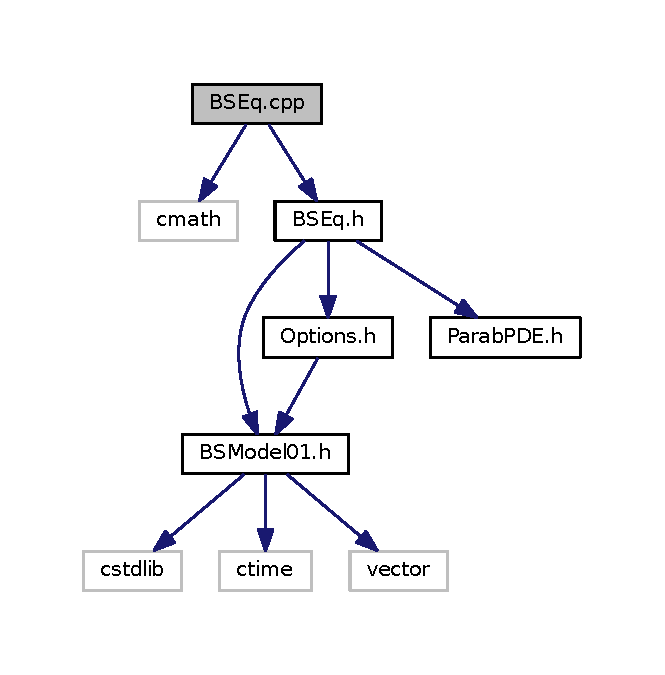
\includegraphics[width=319pt]{BSEq_8cpp__incl}
\end{center}
\end{figure}


\subsection{Detailed Description}
A typical reason for studying parabolic partial differential equations in finance is the Black–-\/\+Scholes equation.

Let $ S(t) $ denote the price at time $ t $ of the underlying asset under the Black–-\/\+Scholes equation. Suppose that at time $ t $ the price of a financial derivative $ H(t) $ can be expressed using a function $ u $, defined as\+: \[ H(t) = u(t, S (t)). \] If $ u $ is a $ C^{1,2} $ function on $ [0,T)\times \mathbb{R} $, then the Black--Scholes equation can be used to solve for $ u $.

When $ u(t, S(t)) $ is the value of an option with expiry date $ T $ and payoff $ H(T) = h(S(T)) $, then $ u(T, S(T)) = h(S(T)) $, hence the terminal condition is \[ u(T, z) = h(z). \] The lower and upper boundary conditions depend on the type of the option we wish to price. They can usually be derived from heuristic or arbitrage arguments.

For example, for a {\bfseries put option} with expiry date $ T $ and strike price $ K $, if $ S(t) $ is high, then the option is practically worthless since it is unlikely to be exercised. This means that we can consider a sufficiently large $ z_u $ and set\+: \[ u(t, zu) = h^{put}_u(t) = 0. \] Also, if $ S(t) $ is close to zero, then we can assume that we are almost certain to exercise the put at expiry and obtain a payoff close to $ K $. Considering a sufficiently small positive $ z_l $ we can therefore set\+: \[ u(t, zl) = h^{put}_l(t) = exp(-r(T - t))K. \]

\begin{DoxyWarning}{Warning}
This code is also listed and fully explained in the book $\ast$$\ast$\+Numerical Methods in Finance with C++$\ast$$\ast$ by Maciej Capiński and Tomasz Zastawniak, published in September 2012.
\end{DoxyWarning}
\begin{DoxyAuthor}{Author}
\+: Eduardo J. Sanchez (ejspeiro) -\/ ejspeiro at gmail dot com 
\end{DoxyAuthor}


Definition in file \hyperlink{BSEq_8cpp_source}{B\+S\+Eq.\+cpp}.

